\documentclass[a4paper,12pt]{article}
\usepackage[indonesian]{babel}
\usepackage{graphicx}
\usepackage{multirow}
\usepackage{enumitem}
\usepackage{listings}
\usepackage{wrapfig}
\usepackage[T1]{fontenc}
\usepackage{inconsolata}
\usepackage{lipsum}
\usepackage{adjustbox}


\usepackage{color}
\usepackage[table]{xcolor}
\definecolor{lightgray}{rgb}{0.95, 0.95, 0.95}
\definecolor{darkgray}{rgb}{0.4, 0.4, 0.4}
%\definecolor{purple}{rgb}{0.65, 0.12, 0.82}
\definecolor{editorGray}{rgb}{0.95, 0.95, 0.95}
\definecolor{editorOcher}{rgb}{1, 0.5, 0} % #FF7F00 -> rgb(239, 169, 0)
\definecolor{editorGreen}{rgb}{0, 0.5, 0} % #007C00 -> rgb(0, 124, 0)
\definecolor{orange}{rgb}{1,0.45,0.13}		
\definecolor{olive}{rgb}{0.17,0.59,0.20}
\definecolor{brown}{rgb}{0.69,0.31,0.31}
\definecolor{purple}{rgb}{0.38,0.18,0.81}
\definecolor{lightblue}{rgb}{0.1,0.57,0.7}
\definecolor{lightred}{rgb}{1,0.4,0.5}
\usepackage{upquote}
\usepackage{listings}
% CSS
\lstdefinelanguage{CSS}{
  keywords={color,background-image:,margin,padding,font,weight,display,position,top,left,right,bottom,list,style,border,size,white,space,min,width, transition:, transform:, transition-property, transition-duration, transition-timing-function},	
  sensitive=true,
  morecomment=[l]{//},
  morecomment=[s]{/*}{*/},
  morestring=[b]',
  morestring=[b]",
  alsoletter={:},
  alsodigit={-}
}

% JavaScript
\lstdefinelanguage{JavaScript}{
  morekeywords={typeof, new, true, false, catch, function, return, null, catch, switch, var, if, in, while, do, else, case, break},
  morecomment=[s]{/*}{*/},
  morecomment=[l]//,
  morestring=[b]",
  morestring=[b]'
}

\lstdefinelanguage{HTML5}{
  language=html,
  sensitive=true,	
  alsoletter={<>=-},	
  morecomment=[s]{<!-}{-->},
  tag=[s],
  otherkeywords={
  % General
  >,
  % Standard tags
	<!DOCTYPE,
  </html, <html, <head, <title, </title, <style, </style, <link, </head, <meta, />,
	% body
	</body, <body,
	% Divs
	</div, <div, </div>, 
	% Paragraphs
	</p, <p, </p>,
	% scripts
	</script, <script,
  % More tags...
  <canvas, /canvas>, <svg, <rect, <animateTransform, </rect>, </svg>, <video, <source, <iframe, </iframe>, </video>, <image, </image>, <header, </header, <article, </article
  },
  ndkeywords={
  % General
  =,
  % HTML attributes
  charset=, src=, id=, width=, height=, style=, type=, rel=, href=,
  % SVG attributes
  fill=, attributeName=, begin=, dur=, from=, to=, poster=, controls=, x=, y=, repeatCount=, xlink:href=,
  % properties
  margin:, padding:, background-image:, border:, top:, left:, position:, width:, height:, margin-top:, margin-bottom:, font-size:, line-height:,
	% CSS3 properties
  transform:, -moz-transform:, -webkit-transform:,
  animation:, -webkit-animation:,
  transition:,  transition-duration:, transition-property:, transition-timing-function:,
  }
}

\lstdefinestyle{htmlcssjs} {%
  % General design
%  backgroundcolor=\color{editorGray},
  basicstyle={\footnotesize\ttfamily},   
  frame=b,
  % line-numbers
  xleftmargin={0.75cm},
  numbers=left,
  stepnumber=1,
  firstnumber=1,
  numberfirstline=true,	
  % Code design
  identifierstyle=\color{black},
  keywordstyle=\color{blue}\bfseries,
  ndkeywordstyle=\color{editorGreen}\bfseries,
  stringstyle=\color{editorOcher}\ttfamily,
  commentstyle=\color{brown}\ttfamily,
  % Code
  language=HTML5,
  alsolanguage=JavaScript,
  alsodigit={.:;},	
  tabsize=2,
  showtabs=false,
  showspaces=false,
  showstringspaces=false,
  extendedchars=true,
  breaklines=true,
}
\lstset{
    frame=single,
    breaklines=true,
}
%

\graphicspath{ {./img/} }
\begin{document}
\title{ {\Large Laporan Praktikum}\\ Pemrograman Web Client\\{\Large Pertemuan 3}}

\author{Aldzikri Dwijayanto Prathama 
	\\195410189
	\\Informatika}
\makeatletter
\begin{titlepage}
	\begin{center}
		{\huge \bfseries \@title }\\[14ex]
		
\includegraphics[scale=.8]{logo}\\[4ex]
		{\large \@author}\\[12ex]
		{\large \bfseries {SEKOLAH TINGGI MANAJEMEN INFORMATIKA DAN KOMPUTER
				AKAKOM YOGYAKARTA}}
	\end{center}


%{\large \@date} 
\end{titlepage}
\makeatother
%\maketitle
\newpage
\tableofcontents
\newpage
\section{Tujuan}
\begin{enumerate}
    \item Menuliskan CSS sesuai aturan (properti dan nilai)
    \item Menuliskan selektor tag
    \item Menuliskan selektor id
    \item Menuliskan selektor class
    \item Menuliskan script internal style
    \item Menuliskan script eksternal style
    \item Menuliskan inline style
\end{enumerate}
\section{Dasar Teori}
CSS (Cascading Style Sheets) adalah script program yang digunakan untuk mengatur
tampilan website, misalnya warna body , jenis serta ukuran font, layout website.
Perintah html hanya mampu mengatur tampilan untuk satu halaman site sedangkan CSS
mampu mengontrol tampilan banyak halaman sekaligus. CSS tidak dikategorikan sebagai
bahasa pemrograman karena di dalamnya tidak ada struktur kontrol (percabangan,
perulangan, array dll). CSS dapat ditambahkan ke dalam HTML dengan 3 cara:
\begin{enumerate}[label=\alph*.]
    \item inline : melalui atribut “style” pada elemen Html
    \item internal : melalui tag <style> yang diletakkan di dalam tag <Head>
    \item eksternal : CSS disimpan pada sebuah file tersendiri dengan ekstensi *.css
\end{enumerate}

\newpage

\section{Pembahasan}
\subsection{Praktik}
\subsubsection{Praktik 1}
\begin{lstlisting}
<!DOCTYPE html>
<html>
    <head>
        <style>
            body{
                background-color: linen;
            }
            h1 {
                color: green;
                margin-left:40px;
            }
            p{
                color: red;
                margin-left:20px;
            }
        </style>
    </head>
    <body>
        <h1>STMIK AKAKOM</h1>
        <p>Alamat: Jl.Janti no.143, 
        Jaranan, Karang Jambe, 
        Kec. Banguntapan, Bantul, DIY 55918</p>

        <p>Telepon: (0274) 486664</p>
    </body>
</html>
\end{lstlisting}
Pada dokumen html tersebut, terdapat CSS dengan jenis internal, karena script css tersebut 
dimasukkan ke dalam tag <head>. Dari syntax css di atas dari selektornya dikeathui elemen 
yang akan diatur adalah elemen body yang diatur backgroundnya menjadi warna linen. Dan elemen 
h1 dan p diatur warna dan marginnya. Jika dibuka di browser tampilannya seperti berikut:
\begin{center}
    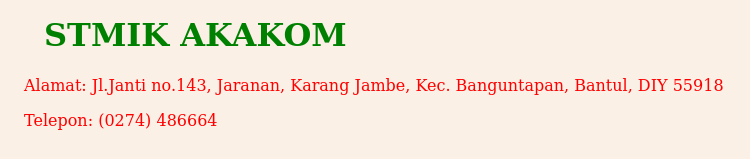
\includegraphics[width=\linewidth]{1.png}
\end{center}

\subsubsection{Praktik 2}
\begin{lstlisting}
<!DOCTYPE html>
<html>
    <body>
    <h1 style="color:blue;text-align:center;">STMIK AKAKOM</h1>
    <p style="color:red;text-align:center">Telepon: (0274) 486664</p>
    </body>
</html>
\end{lstlisting}

Dokumen html tersebut memiliki CSS secara inline, karena dimasukkan langsung di elemen yang
 akan diatur tampilannya.
 \begin{center}
     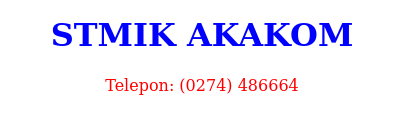
\includegraphics[width=\linewidth]{2.png}
 \end{center}

 \subsubsection{Praktik 3}
 Pada praktik 3 dibuat dokumen html, yang script CSS nya terpisah, Pertama 

\newpage

\end{document}
